\chapter{Desenvolvimento} \label{chap:desen}

\hspace{5mm} Nesta secção será ilustrada a configuração de referência obtida juntamente com os seus resultados. De seguida serão ilustrados quais as alterações realizadas às configurações da base de dados PostegreSQL e quais as otimizações de desempenho obtidas com essas mesmas alterações.

\section{Configuração de Referência} \label{sec:refBase}

%Possibilidade de dividir em subsection para configuração e avaliação da configuração

%Não pq são várias fases do desenvolvimento

\hspace{5mm} Para determinar a configuração de referência foram realizados vários testes. Na configuração da aplicação EscadaTPC-C variou-se tanto o número de \textbf{warehouses}, bem como \textbf{número de clientes por warehouse} no ficheiro worload-proprieties. Nas máquinas variou-se os seus recursos: número de \textbf{CPUs}, \textbf{RAM} e \textbf{ROM}.

\hspace{5mm} De forma a \textbf{maximizar o tempo disponível} foram instaladas e configuradas todas as dependências (postgresql e TPC-C) para realizar os testes numa máquina, de seguida foi criado um \textbf{snapshot} e criadas mais 8 máquinas equivalentes. Desta forma foi possível efetuar 9 testes em \textbf{simultâneo}.

\hspace{5mm} Com o mesmo propóstivo foi criado um bash script - \textbf{start\_bd.sh} - que cria a base de dados, percorre os scripts forncecidos pela equipa docente para a criação de tabelas, indices, etc; faz o povoamento (load.sh) e corre o benchmark (run.sh). Foi também criado um \textbf{makefile} que move os ficheiros .dat para uma pasta de resultados e remove ficheiros que já não são relevantes. Tudo isto contribuiu para \textbf{automatizar} a realização de testes.  

\hspace{5mm} A \textbf{monotorização} da utilização de CPU e memória RAM foi obtida através do serviço  \textcolor{blue}{\href{https://cloud.google.com/stackdriver/}{stackdriver}} fornecido pela Google. Desta forma, para cada máquina, foi possível registar as respetivas \textbf{métricas} e analisar as mesmas através de gráficos, tal como a seguinte figura ilustra.

%imagem
\begin{figure}[H]
    \centering
    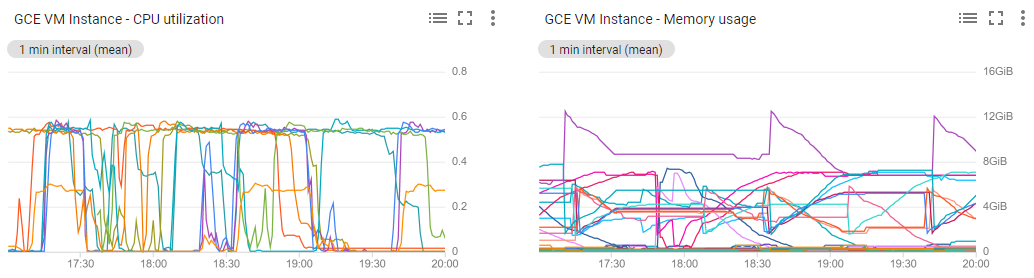
\includegraphics[scale=0.65]{imagens/charts_usage.PNG}
    \caption{Monotorização do CPU e RAM.}
    \label{fig:confRef}
\end{figure}

\hspace{5mm} A figura anterior apresenta informação relativa a todas as máquinas, no entanto é possível salientar os recursos de cada máquina \textbf{individualmente} e mesmo obter dados \textbf{temporais}, tal como se segue.

%imagem
\begin{figure}[H]
    \centering
    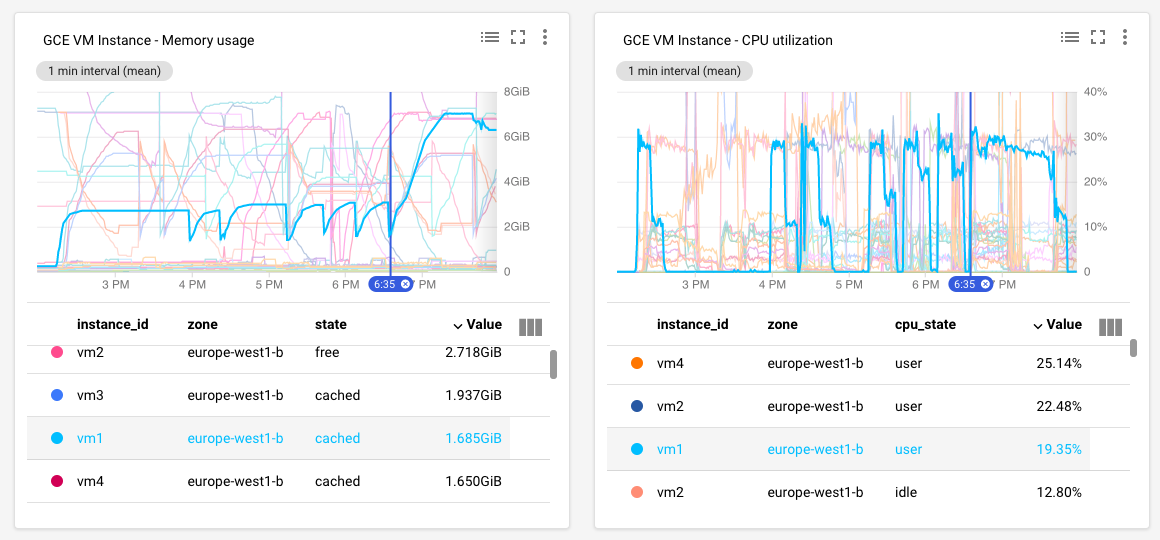
\includegraphics[scale=0.4]{imagens/60w-150c.png}
    \caption{Métricas de CPU e memória RAM (linha azul realçada) da configuração de 60 warehouses e 150 clientes por warehouse na \textbf{vm1} com hora inicial do teste ás 06h35m PM.}
    \label{fig:confRef}
\end{figure}

\hspace{5mm} Através da interpretação das métricas de \textbf{31 testes}, conclui-se que a máquina com resultados mais \textbf{eficientes} para os testes realizados contém os seguintes recursos: \textbf{2 cores}, \textbf{8 GB de RAM} e \textbf{30 GB de SSD} persistente.

\hspace{5mm} Com o hardware anterior determinou-se que a configuração ideal do benchmark TPC-C consiste em em \textbf{70 warehouses} e \textbf{150 clientes}. A utilização de CPU foi cerca de 60\% e foi utilizada cerca de 85\% da memória RAM.

\hspace{5mm} Note-se que era possível aumentar o número de warehouses e os respetivos clientes, no entanto, face à \textbf{limitação de recursos} e \textbf{tempo disponível para os testes}, conclui-se que a configuração anterior é a ideal, sendo suficiente para apresentar possíveis melhorias de desempenho.

\hspace{5mm} Com a ajuda do script \textbf{showtpc.py} fornecido pela equipa docente foi possível obter dados de desempenho como o débito, tempo de resposta e taxa de cancelamento de transações.

\newpage
\section{Otimização do Desempenho da Carga Transacional} \label{sec:refOpti}

\hspace{5mm} A otimização no desempenho da carga transacional, usando a configuração de referência, realizou-se com alterações às configurações da base de dados PostgreSQL. Foram alterados alguns paramêtros de configuração, complementados com testes, para verificação da vantagem dessa alteração.

\hspace{5mm}A configuração de referência apenas utiliza cerca de 85\% da RAM como foi referido anteriormente, esta decisão foi propositada uma vez que era de esperar aumentar a quantidade de RAM disponível para os diferentes buffers dos processos do servidor postgresql, desta forma \textbf{tem de existir uma margem diponível}.


\subsection{Parâmetro shared\_buffer}

Em qualquer circustância acessos (leitura e escrita) em memória RAM são \textbf{extremamente mais rápidos} que em disco, desta forma o servidor postgresql usufrui de uma cache denominada de \textbf{shared\_buffer} onde armazena parte de tabelas ou indices temporariamente e realiza operações sobre as mesmas, de seguida, se necessário, volta a escrever os dados em memória presistente.

%imagem
\begin{figure}[H]
    \centering
    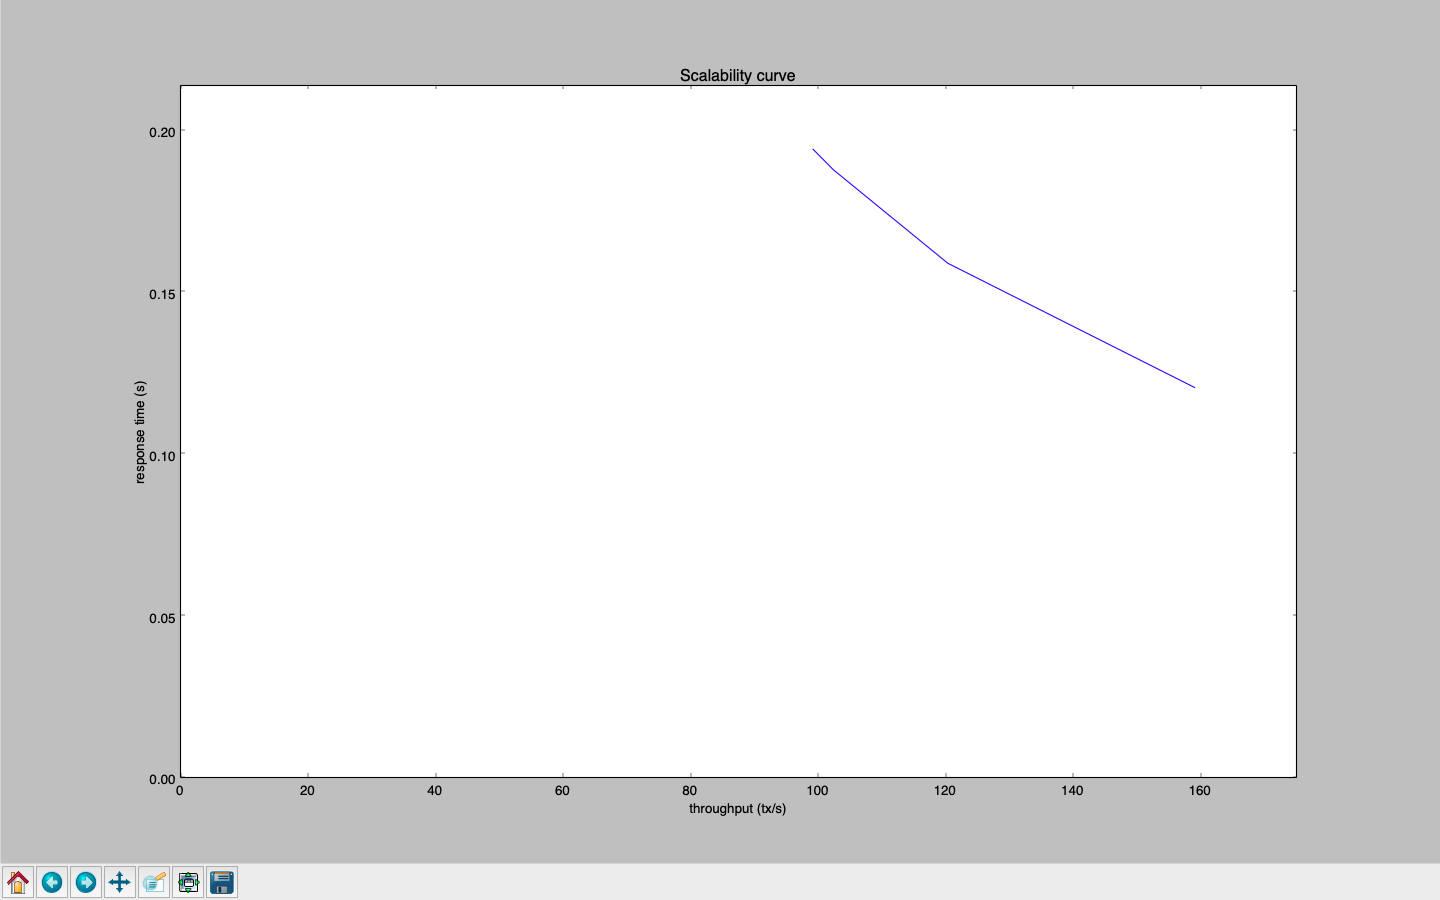
\includegraphics[scale=0.3]{imagens/shared_buffer_scability.png}
    \caption{Escalabilidade do \emph{troughput} para valores do shared\_buffer de 128MB, 256MB, 512MB e 1024MB.}
    \label{fig:sharedbuffer}
\end{figure}

\hspace{5mm} Apenas com a alteração do parâmetro \textbf{shared\_buffer} de 128MB (padrão) para \textbf{1024MB} foi possível \textbf{aumentar o débito em cerca de 60\%} e o \textbf{tempo de resposta diminuiu em cerca de 40\%}. Também foram realizados testes com 256MB e 512MB como pode ser visualizado na figura \ref{fig:sharedbuffer}, sendo que o melhor valor obtido foi o de 1024MB. \newline

\hspace{5mm} Esta \textbf{melhoria tão acentuada} justifica-se uma vez que com mais memória RAM disponível para este parâmetro, os processos do servidor postgresql não necessitam de aceder ao disco (memória lenta) tantas vezes.

\hspace{5mm} Importante referir, que provavelmente para valores de \textbf{shared\_buffer} maiores do que 1024MB \textbf{(até a valores próximos do limite de RAM)}, poderia se obter ainda melhores resultados. No entanto, devido à falta de tempo para realização de mais testes, e como já se obteve melhoria aceutado em relação à configuração padrão, decidiu-se utilizar este valor.

\subsection{Parâmetro work\_mem}

\hspace{5mm}  Este parâmetro controla a quantidade de memória RAM alocada, tipicamente, \textbf{por cada} operação de ordenação (ORDER BY, DISTINCT, etc). Note-se que podem existir muitas operações deste tipo a correr em simultâneo no servidor, desta forma a quantide de RAM disponível para cada operação \textbf{não pode ser muito grande, caso contrário a RAM é esgotada rapidamente}, tornando o sistema operativo e todos os processos mais lentos.
\begin{figure}[H]
    \centering
    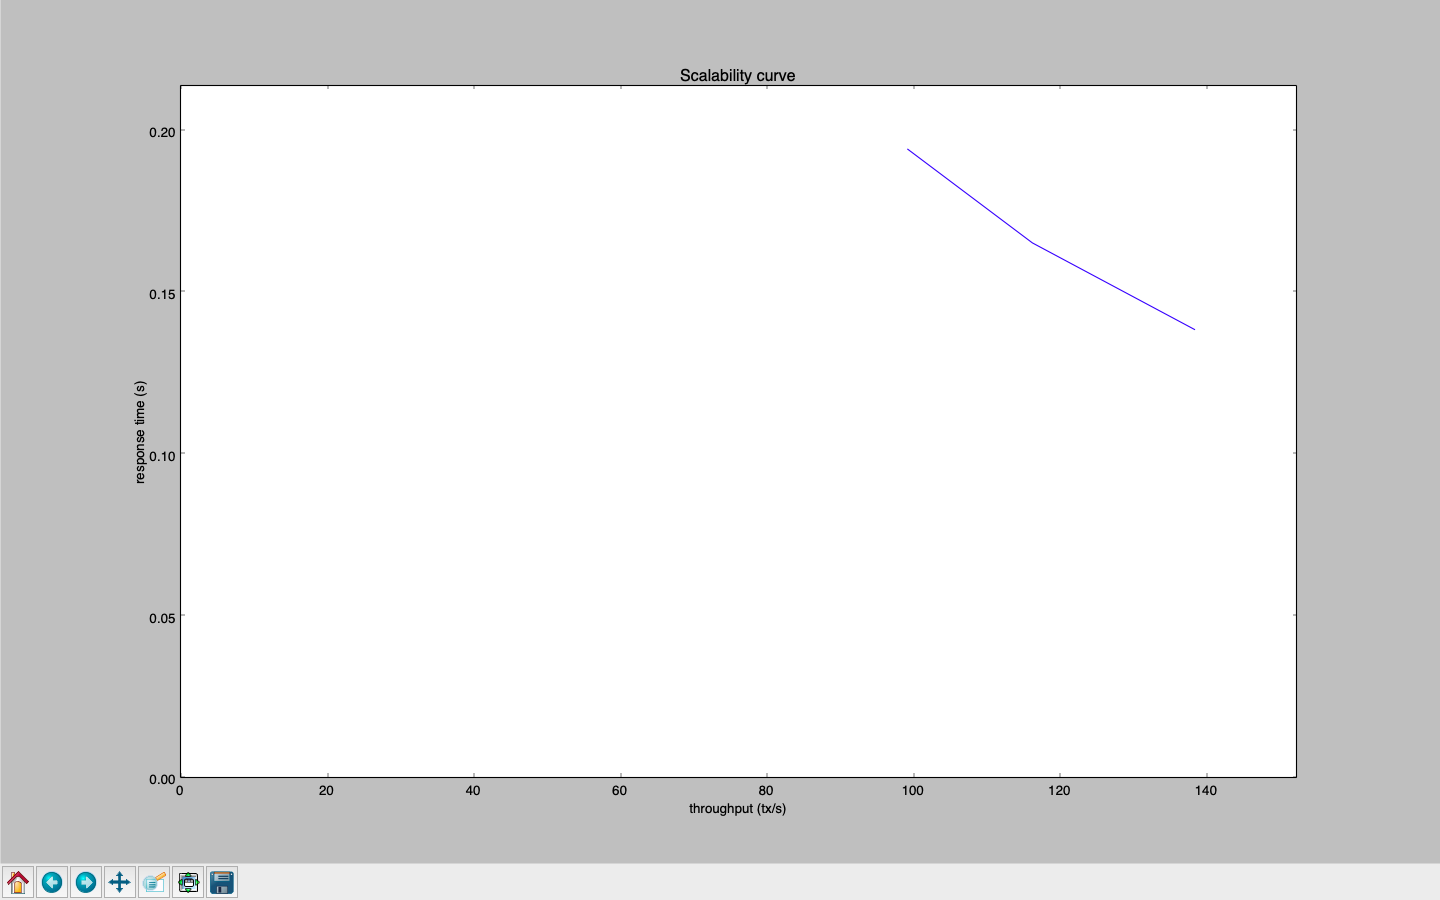
\includegraphics[scale=0.3]{imagens/work-mem-4MB-8MB-16MB.png}
    \caption{Escalabilidade do \emph{troughput} para valores do work\_mem de 4MB, 8MB, e 16MB.}
    \label{fig:exemplo}
\end{figure}

\hspace{5mm} Com a alteração do parâmetro \textbf{work\_mem} também foram obtidos ganhos quando alterado de 4MB para 8MB, 16MB, 32MB e 64MB, sendo que destes o que teve a melhor otimização de desempenho foi o valor de \textbf{16MB}.

\hspace{5mm} Note-se que para valores de 32MB de 64MB os resultados obtidos foram piores do que com 16MB, isto justifica-se uma vez que esta quantidade de RAM é alocada \textbf{por cada} operação, tal como referido anteriomente, desta forma, provavelmente valores de 32MB e 64MB são suficientes para existir \textbf{escassez de RAM tornando os processos mais lentos}. 

\newpage

\hspace{5mm} Os resultados que demonstram este \textbf{declínio de desempenho} apresentam-se de seguida na figura \ref{fig:exemplo}. O débito (throughput) diminui e o tempo de resposta aumentou em relação aos teste realizados com 16MB.

\begin{figure}[H]
    \centering
    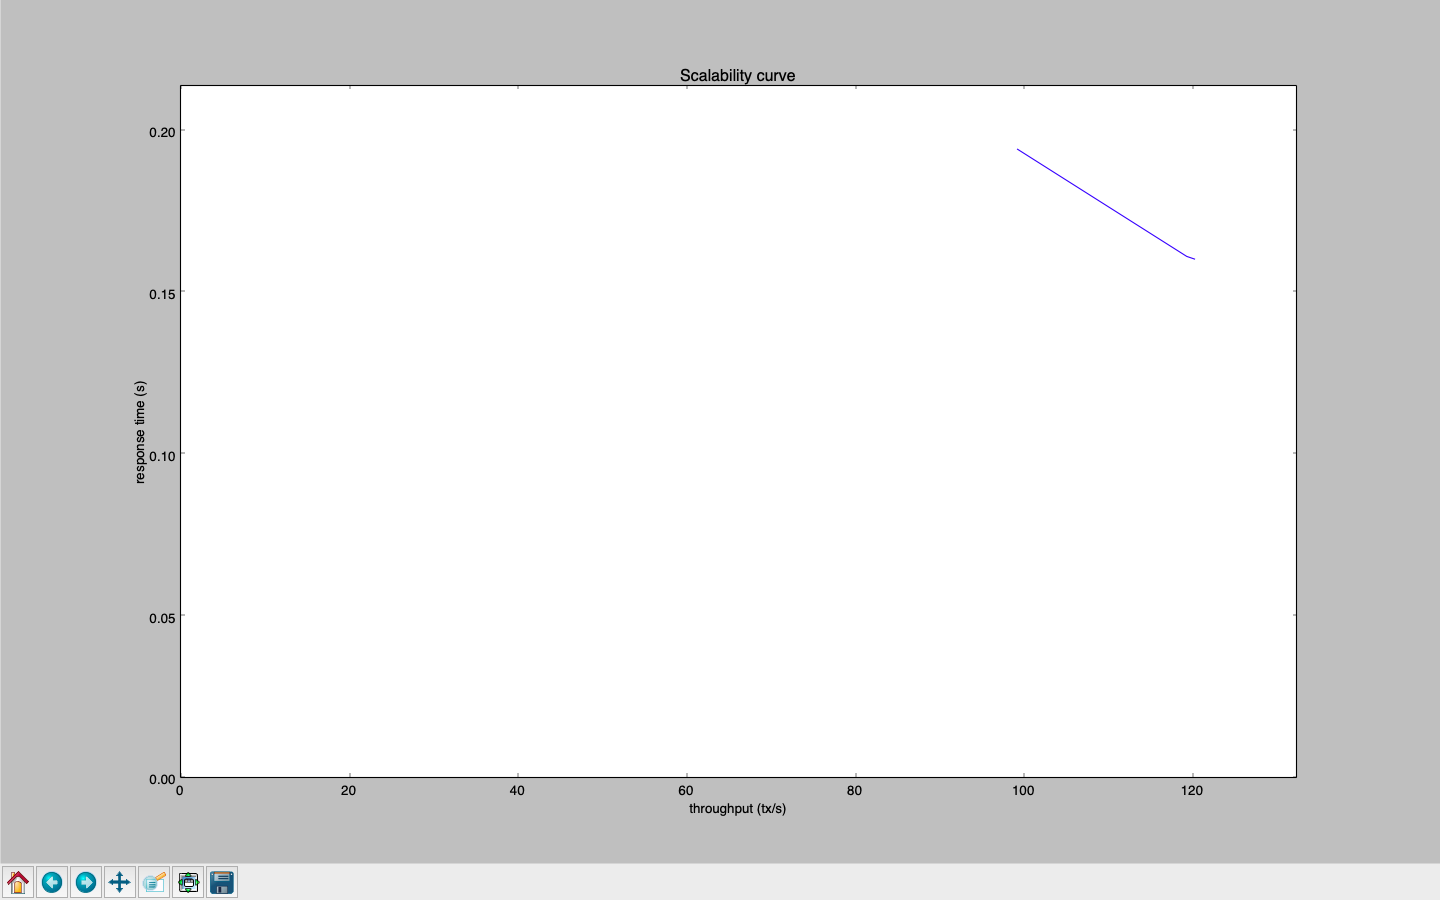
\includegraphics[scale=0.3]{imagens/work-mem-4MB-32MB-64MB.png}
    \caption{Escalabilidade do \emph{troughput} para valores do work\_mem de: 4MB, 32MB e 64MB.}
    \label{fig:exemplo}
\end{figure}

\newpage
\subsection{Parâmetro wal\_buffer}

\hspace{5mm} Este parâmetro controla a quantidade de RAM disponível para armazenar os WAL - \textbf{W}rite \textbf{A}head \textbf{L}ogs. Todas as alterações aos dados são registadas nestes logs para que, caso o sevidor falhe, seja possível reconstruir os dados totalmente. Desta forma esta porção de memória RAM está constantemente a ser preenchida e quando cheia é copiada para memória presistente. Enquanto está a ser copiada, todos os processos de escrita ficam em espera (para registar os seus logs).

%imagem
\begin{figure}[H]
    \centering
    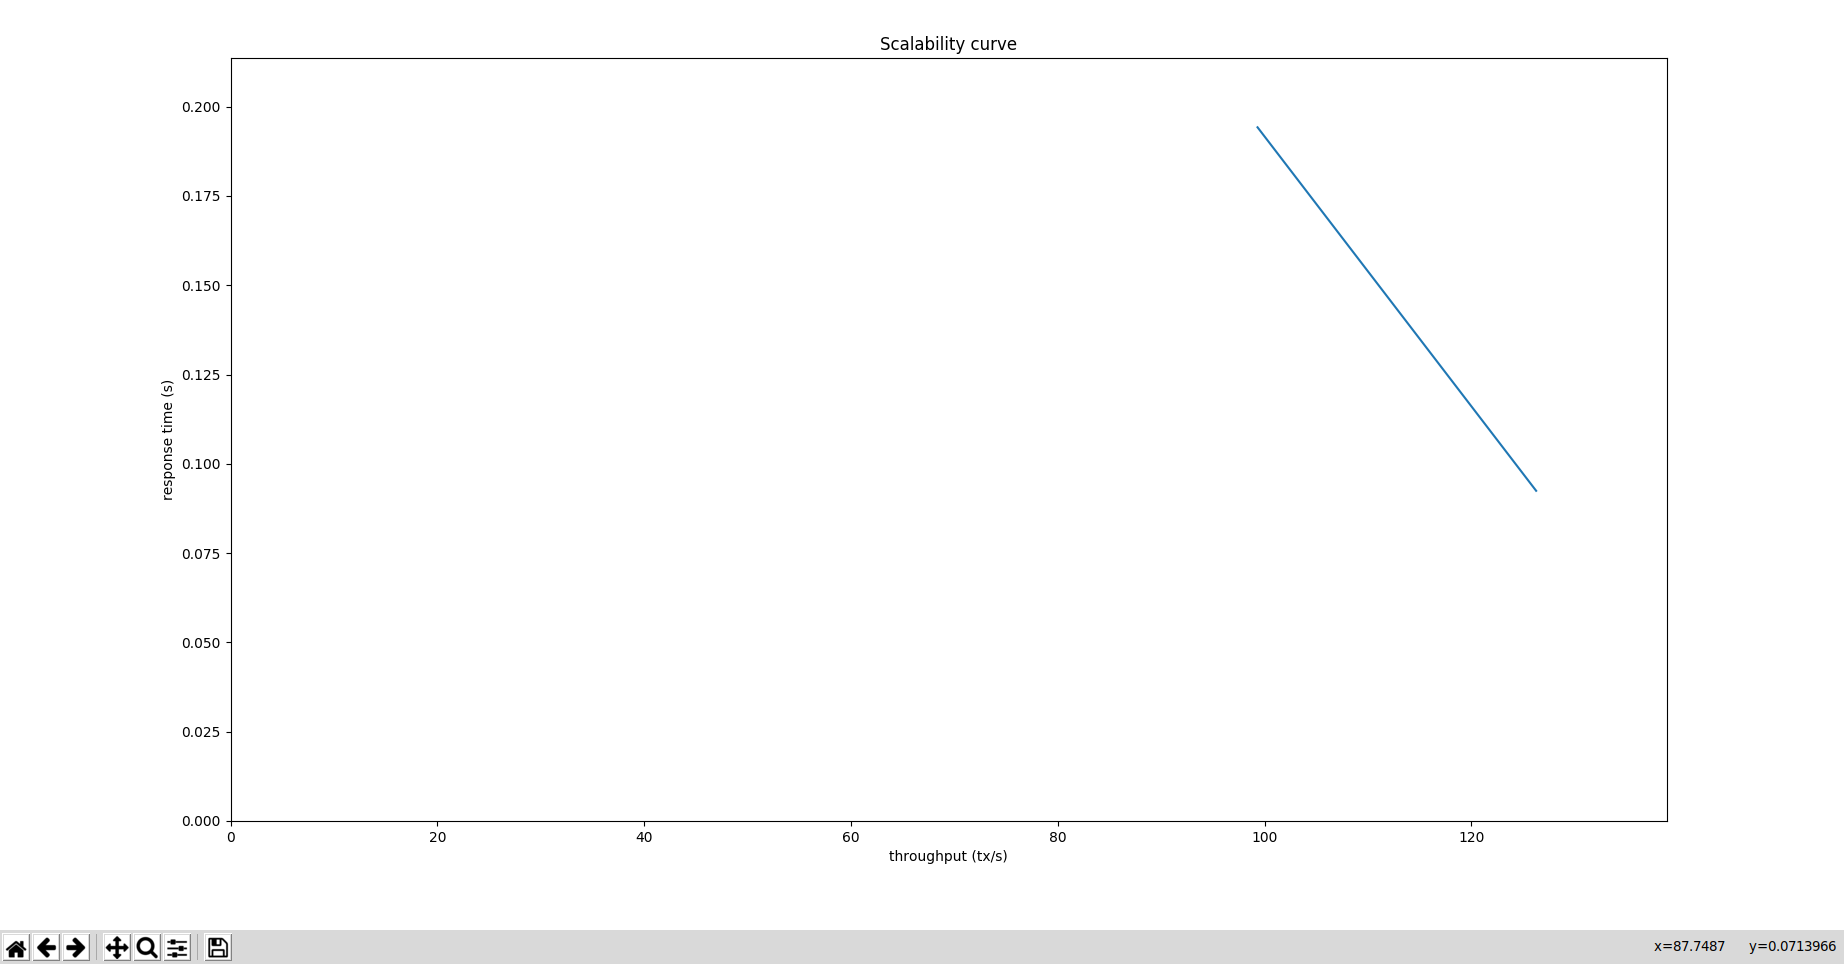
\includegraphics[scale=0.25]{imagens/wall_buffer.png}
    \caption{Escalabilidade do \emph{troughput} para valores do wal\_buffers: padrão e 32MB.}
    \label{fig:exemplo}
\end{figure}

\hspace{5mm} Como se pode observar no gráfico anterior, com \textbf{32MB} de wal\_buffer o débito aumentou em cerca de 27.13\% e o tempo de resposta diminui muito. Esta otimização justifica-se uma vez que o buffer \textbf{demora mais tempo a ficar totalmente preenchido, desta forma o número de vezes que os processos ficam à espera (da cópia da RAM para o disco) é menor}.

\newpage
\subsection{Configuração ideal}

\hspace{5mm} Após alterar cada parâmetro individualmente e obter melhorias em todos os testes, decidiu-se realizar um teste final com os 3 parêmetros modificados. Desta forma a configuração ideal consiste em:

\begin{itemize}
    \item shared\_buffer = 1024 MB
    \item work\_mem = 16 MB
    \item wall\_buffer = 32 MB
\end{itemize}

Consequentemente o \textbf{débito aumentou em cerca de 70.83\%} e o \textbf{tempo de resposta diminui}, tal como se pode observar no seguite gráfico.

%imagem
\begin{figure}[H]
    \centering
    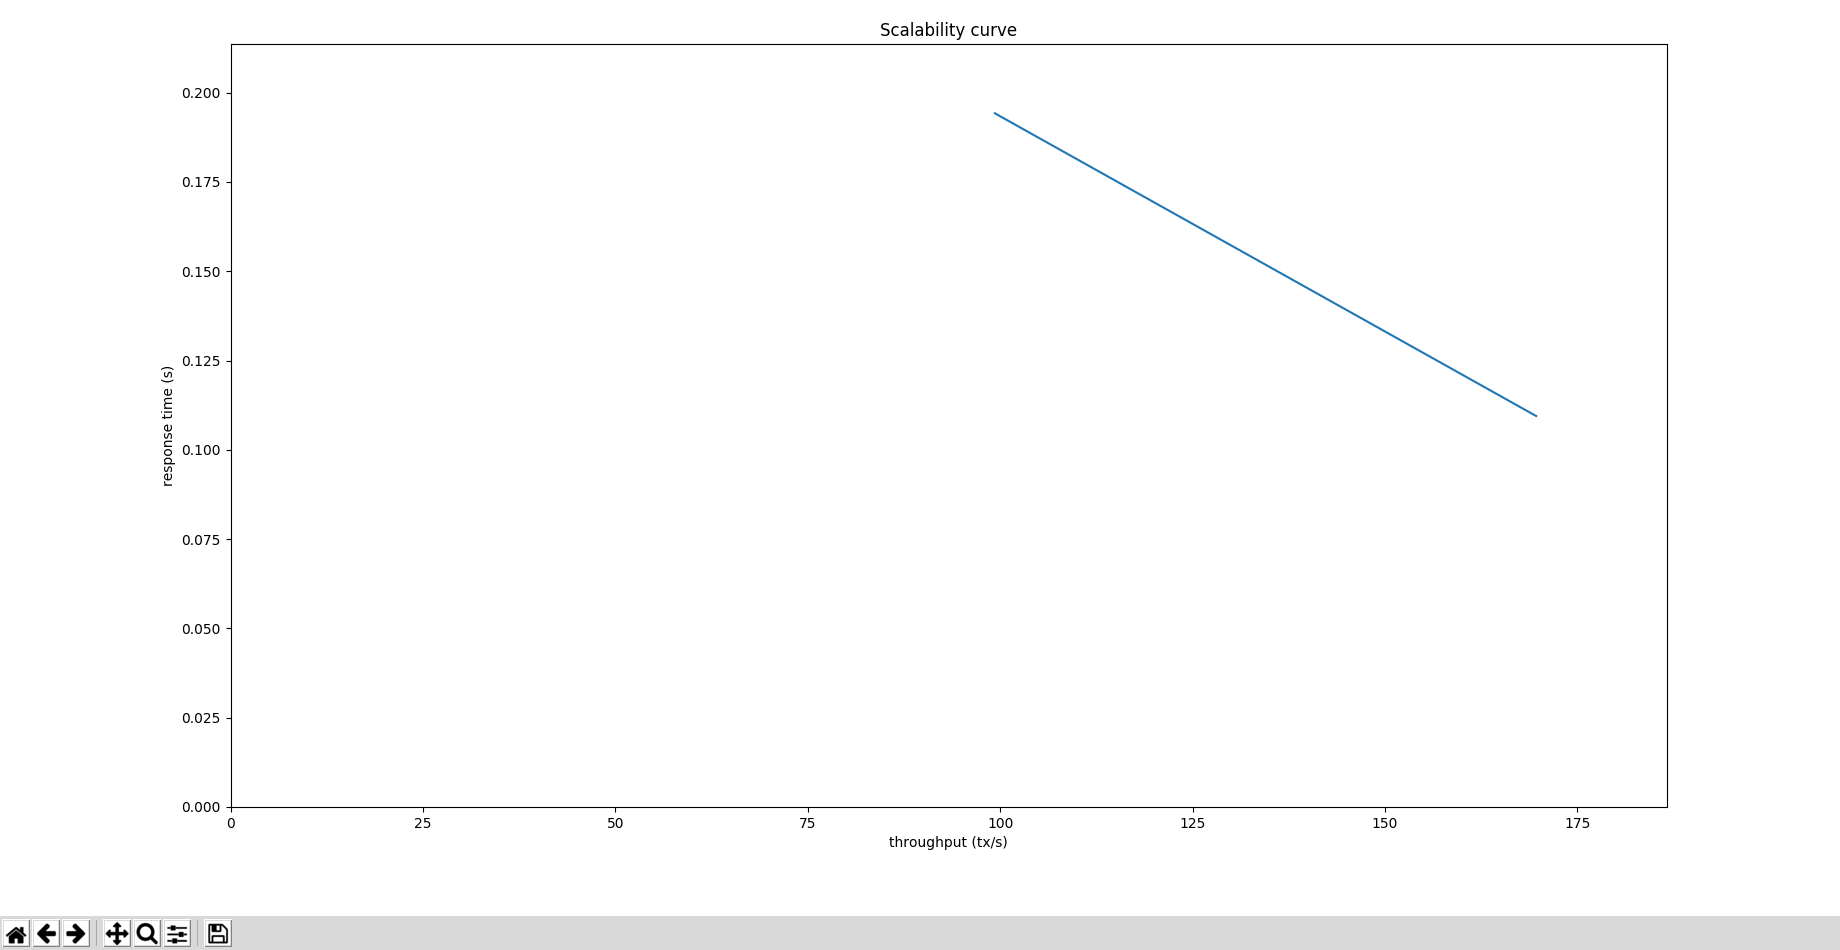
\includegraphics[scale=0.25]{imagens/otima.png}
    \caption{Escalabilidade do \emph{troughput} com configuração final otimizada.}
    \label{fig:exemplo}
\end{figure}

\newpage
%Modificar o nome
\section{Otimização de Desempenho de Queries Analíticas}

\hspace{5mm} Este capítulo aborda as téncias utilizadas para otimizar o desempenho das queries analíticas fornecidas pela equipa docente.

\hspace{5mm} Tal como referido nas aulas a introdução de \textbf{redudância} através de \textbf{indices} e \textbf{vistas materializadas} é espectável que seja suficiente para otimizar com grande relância todas as queries.

\hspace{5mm} As views materializadas devem ser criadas quando uma determinada queire é \textbf{demasiado lenta} a processar ao ponto de ser intolerável esperar esse tempo cada vez que a mesma é executada. 

\hspace{5mm} No entanto como o resultado das views materializas \textbf{é gerado no momento que a mesma é criada}, a informação contida nestas views pode não ser a mais atual quando é evocada. Por este motivo este tipo de views deve ser associado a informação que raramente é alterada ou a sua alteração não tem impacto crítico na validade dos resultados.

\hspace{5mm} Posto isto, inicialmente, começou-se por gerar o plano da queire nº1 através do comando \textbf{explain} no postgres. 

\hspace{5mm} Verificamos que a querie utilizava o algoritmo NLJ - \textbf{N}ested \textbf{L}oop \textbf{J}oin - para unir a tabelas, no entanto tal como referido nas aulas em muitos casos este algoritmo \textbf{pode não ser o ótimo} uma vez que caso a primeira tabela tenha N linhas, o algoritmo vai percorrer N vezes a segunda tabela com complexidade \textbf{N$^2$}, tendo a vantagem de necessitar menor memória RAM para a sua execução, uma vez que apenas necessita de uma linha de cada tabela em cada momento.

\hspace{5mm} Desta forma decidiu-se desativar o algoritmo NLJ nos ficheiros de configuração do postgres. Foram realizados alguns testes medindo o tempo que cada querie demorava a responder utilizando o comando \textbf{timming} e verificou-se que, \textbf{ao contrário do espectável pelo grupo}, o tempo de processamento aumentou.  

\hspace{5mm} Analisando ainda a querie nº1 decidiu-se que no sublinhado a azul encontra-se a sub-querie transformada em view materializada e a verde encontra-se as colunas transformadas indices.

%imagem
\begin{figure}[H]
    \centering
    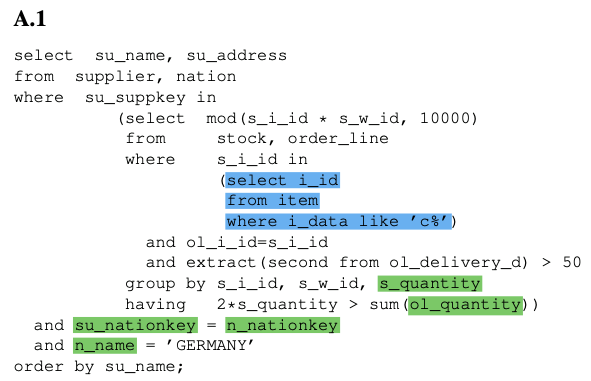
\includegraphics[scale=0.5]{imagens/q1.png}
    \caption{Alterações feitas na queri 1 (Azul = View Materializada, Verde = index).}
    \label{fig:exemplo}
\end{figure}

\hspace{5mm} Note-se que é possível criar a view materializada a partir da sub-querie referida uma vez os campos \textbf{i\_data} e \textbf{i\_id} da tabela item, á partida, \textbf{não são alterados} e memso que fossem alterados, visto que esta querie é possivlemente apenas executada por membros de administração, não deverá ter grande impacto ter dados desatualizados.

\hspace{5mm} Com a introdução desta view meterializada tivemos \textbf{ganhos significativos}, o tempo de processamento da querie \textbf{reduziu cerca de 138 ms} tal como é possível observar na seguinte figura.

%imagem
\begin{figure}[H]
    \centering
    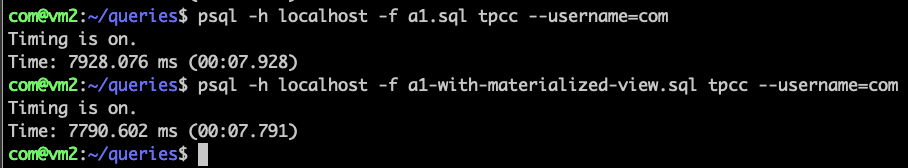
\includegraphics[scale=0.5]{imagens/q1_view_mat.png}
   \caption{Otimização de desempenho com introdução da view materializada.}
    \label{fig:exemplo}
\end{figure}

\hspace{5mm} Em primeira análise pode-se pensar que 138 ms é um ganho sem grande impacto mas se se multiplicar este valor por inúmeros clientes simultâneamente a evocar esta querie, tal como nos testes do benchamark TPC-C, provavelmente os ganhos são significativos.

\hspace{5mm} De seguida foi testada a introdução dos indices anteriormente referidos e medido o tempo de processamento com esta alteração. As seguintes figuras ilustram a melhoria em tempo de processamento ganho com a introdução destes indices.

%imagem
\begin{figure}[H]
    \centering
    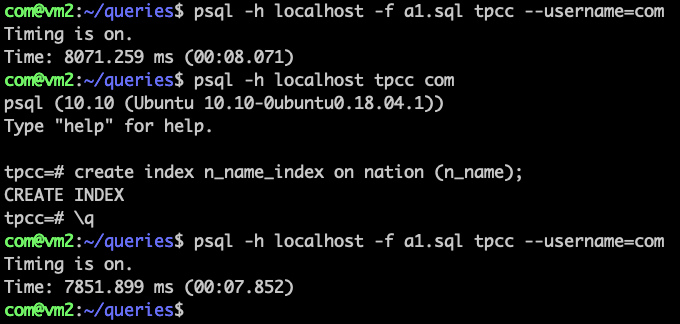
\includegraphics[scale=0.5]{imagens/q1_index_1.png}
    \caption{Testes antes e depois da inserção do index \textbf{n\_name_index}.}
    \label{fig:exemplo}
\end{figure}

%imagem
\begin{figure}[H]
    \centering
    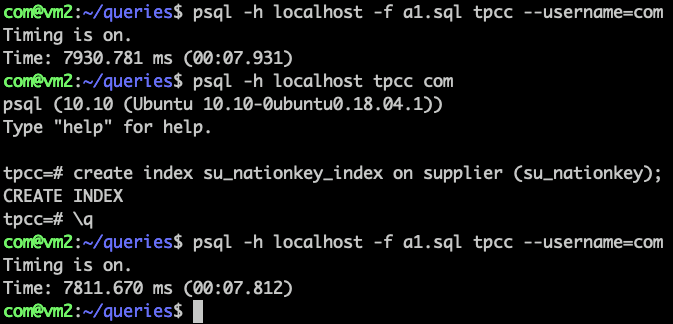
\includegraphics[scale=0.5]{imagens/q1_index_2.png}
    \caption{Testes antes e depois da inserção do index \textbf{su\_nationkey\_index}.}
    \label{fig:exemplo}
\end{figure}

%imagem
\begin{figure}[H]
    \centering
    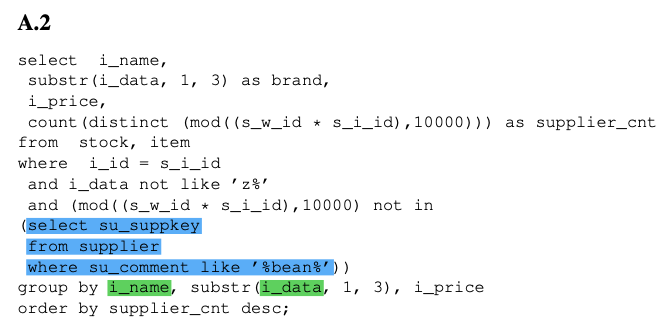
\includegraphics[scale=0.5]{imagens/a2.png}
    \caption{Alterações feitas na queri 2 (Azul = View Materializada, Verde = index).}
    \label{fig:exemplo}
\end{figure}

%imagem
\begin{figure}[H]
    \centering
    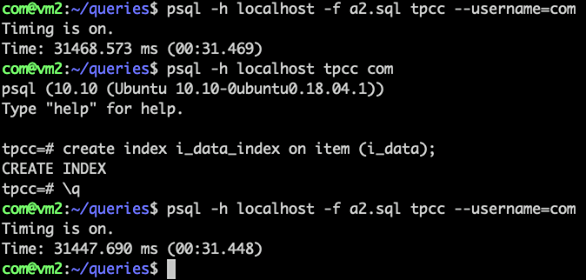
\includegraphics[scale=0.5]{imagens/a2-1.png}
     \caption{Testes antes e depois da inserção do index \textbf{i\_data\_index}.}
    \label{fig:exemplo}
\end{figure}

%imagem
\begin{figure}[H]
    \centering
    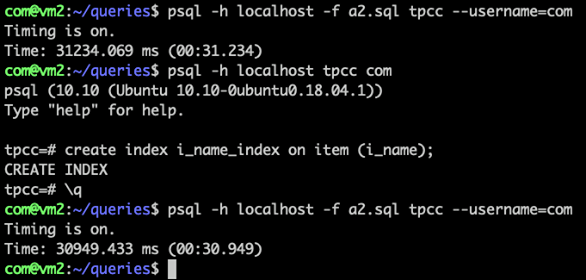
\includegraphics[scale=0.5]{imagens/a2-2.png}
     \caption{Testes antes e depois da inserção do index \textbf{i\_name\_index}}
    \label{fig:exemplo}
\end{figure}